% Created 2021-11-13 sáb 20:40
% Intended LaTeX compiler: pdflatex
\documentclass[aspectratio=169, xcolor={usenames,svgnames,dvipsnames}]{beamer}
\usepackage[utf8]{inputenc}
\usepackage[T1]{fontenc}
\usepackage{graphicx}
\usepackage{grffile}
\usepackage{longtable}
\usepackage{wrapfig}
\usepackage{rotating}
\usepackage[normalem]{ulem}
\usepackage{amsmath}
\usepackage{textcomp}
\usepackage{amssymb}
\usepackage{capt-of}
\usepackage{hyperref}
\usepackage{color}
\usepackage{listings}
\usepackage{mathpazo}
\usepackage{gensymb}
\usepackage{amsmath}
\usepackage{diffcoeff}
\usepackage{steinmetz}
\usepackage{mathtools}
\bibliographystyle{plain}
\usepackage{siunitx}
\sisetup{output-decimal-marker=comma}
\DeclareSIUnit{\watthour}{Wh}
\hypersetup{colorlinks=true, linkcolor=Blue, urlcolor=Blue}
\renewcommand{\thefootnote}{\fnsymbol{footnote}}
\newcommand{\laplace}[1]{\mathbf{#1}(\mathbf{s})}
\newcommand{\slp}{\mathbf{s}}
\newcommand{\fasor}[1]{\mathbf{#1}(\omega)}
\newcommand{\atan}{\mathrm{atan}}
\parskip=5pt
\usetheme{Boadilla}
\usecolortheme{rose}
\usefonttheme{serif}
\author{Ana Fernández-Guillamón}
\date{}
\title{Sistemas trifásicos}
\setbeamercolor{alerted text}{fg=blue!50!black} \setbeamerfont{alerted text}{series=\bfseries}
\AtBeginSubsection[]{\begin{frame}[plain]\tableofcontents[currentsubsection,sectionstyle=show/shaded,subsectionstyle=show/shaded/hide]\end{frame}}
\AtBeginSection[]{\begin{frame}[plain]\tableofcontents[currentsection,hideallsubsections]\end{frame}}
\beamertemplatenavigationsymbolsempty
\setbeamertemplate{footline}[frame number]
\setbeamertemplate{itemize items}[triangle]
\setbeamertemplate{enumerate items}[circle]
\setbeamertemplate{section in toc}[circle]
\setbeamertemplate{subsection in toc}[circle]
\hypersetup{
 pdfauthor={Oscar Perpiñán Lamigueiro},
 pdftitle={Sistemas Trifásicos},
 pdfkeywords={},
 pdfsubject={},
 pdfcreator={Emacs 27.1 (Org mode 9.4.6)}, 
 pdflang={Spanish}}
\begin{document}

\maketitle

\section{Introducción}

\begin{frame}{Introducción}
\begin{itemize}
\item Generación, transporte y distribución de energía eléctrica
\item Sistema polifásico de orden $n\equiv n$ fuentes desfasadas $360/n$
\item Instalaciones monofásicas alimentadas por una fase de sistema trifásico
\item Ventajas:
\begin{itemize}
    \item La potencia instantánea es constante, mientras que en uno monofásico es pulsante
    \item La masa de conductor necesaria en un sistema trifásico es un 25\% inferior que en un monofásico para transportar la misma potencia 
\end{itemize}
\end{itemize}
\end{frame}

\begin{frame}{Introducción}{Ondas trifásicas}
  
    \begin{columns}
      \begin{column}{0.5\linewidth}
        \begin{center}
          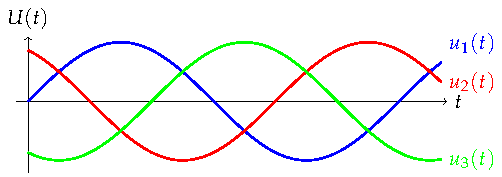
\includegraphics{../figs/TensionesTrifasica.pdf}
        \end{center}
      \end{column}
      \begin{column}{0.5\linewidth}
        \begin{center}
          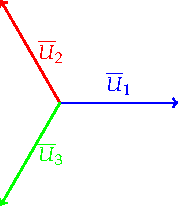
\includegraphics{../figs/FasoresTrifasica.pdf}
        \end{center}
      \end{column}
    \end{columns}
    

\begin{align*}
  u_1(t) = \sqrt{2}\, U \sin(\omega t) & \rightarrow \overline{U}_1 = U\phase{0}\\
  u_2(t) = \sqrt{2}\, U \sin(\omega t + 2\pi/3)& \rightarrow \overline{U}_2 = U\phase{120}\\
  u_3(t) = \sqrt{2}\, U \sin(\omega t - 2\pi/3) & \rightarrow \overline{U}_3 = U\phase{-120}
\end{align*}
\end{frame}

\begin{frame}{Introducción}{Sistemas equilibrados y desequilibrados}
\begin{columns}
\begin{column}{0.3\linewidth}
\alert{Sistema equilibrado}
\begin{itemize}
    \item Igual módulo \alert{y}
    \item Igual desfase
\end{itemize}

\vspace{5mm}
\alert{Sistema desequilibrado}
\begin{itemize}
    \item Diferente módulo \alert{y/o}
    \item Diferente desfase
\end{itemize}
\end{column}
\pause\begin{column}{0.3\linewidth}
\begin{center}
    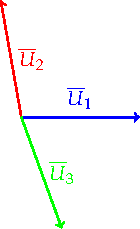
\includegraphics[width=0.7\linewidth]{../figs/fasores_desq1.pdf}
\end{center}
\end{column}
\pause\begin{column}{0.3\linewidth}
\begin{center}
    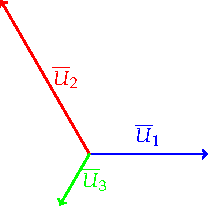
\includegraphics[width=\linewidth]{../figs/fasores_desq2.pdf}
\end{center}
\end{column}
\end{columns}
\end{frame}

\section{Generadores trifásicos}

\begin{frame}{Generadores trifásicos}{Sistema equilibrado}
\begin{columns}
\begin{column}{0.6\columnwidth}
\begin{align*}
  u_1(t) = \sqrt{2}\, U \sin(\omega t) & \rightarrow \overline{U}_1 = U\phase{0}\\
  u_2(t) = \sqrt{2}\, U \sin(\omega t + 2\pi/3)& \rightarrow \overline{U}_2 = U\phase{120}\\
  u_3(t) = \sqrt{2}\, U \sin(\omega t - 2\pi/3) & \rightarrow \overline{U}_3 = U\phase{-120}
\end{align*}
\end{column}
\begin{column}{0.4\columnwidth}
\begin{center}
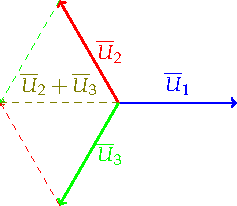
\includegraphics[height=0.5\textheight]{../figs/FasoresSumaCero.pdf}
\[
\boxed{\overline{U}_1 + \overline{U}_2 + \overline{U}_3 = 0}
\]
\end{center}
\end{column}
\end{columns}
\end{frame}

\begin{frame}{Generadores trifásicos}{Equilibrados}
\begin{center}
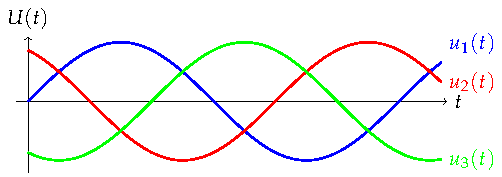
\includegraphics[width=.9\linewidth]{../figs/TensionesTrifasica.pdf}
\end{center}

\[
\boxed{u_1(t) + u_2(t) + u_3(t) = 0}
\]
\end{frame}


\subsection{Tensión de fase y de línea}

\begin{frame}{Tensión de fase y de línea}{Sistema equilibrado}
Tensiones de \alert{fase}: entre fase--neutro (generador), en la impedancia (receptor)
\begin{itemize}
    \item \(\overline{U_A}\), \(\overline{U_B}\), \(\overline{U_C}\) $\equiv U_F$
\end{itemize}

Tensiones de \alert{línea}: entre conductores de la línea
\begin{itemize}
    \item \(\overline{U_{AB}}\), \(\overline{U_{BC}}\), \(\overline{U_{CA}}\) $\equiv U_L$
\end{itemize}

\begin{columns}
\begin{column}{0.4\columnwidth}
\begin{center}
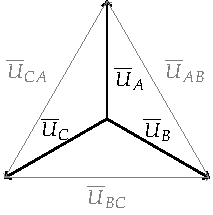
\includegraphics[height=0.4\textheight]{../figs/FasoresTrifasica_ABC.pdf}
\end{center}
\end{column}

\begin{column}{0.6\columnwidth}
\begin{align*}
       \overline{U}_{AB} &= \overline{U}_A - \overline{U}_B\\
       \overline{U}_{BC} &= \overline{U}_B - \overline{U}_C\\
       \overline{U}_{CA} &= \overline{U}_C - \overline{U}_A\\
\cline{1-2}
       \overline{U}_{AB} + \overline{U}_{BC} + \overline{U}_{CA} &= 0     
       \end{align*}
\end{column}
\end{columns}
\end{frame}

\subsection{Secuencia de fases}

\begin{frame}{Secuencia de fases}
\begin{itemize}
\item Orden en que suceden las tensiones de cada fase (p. ej., valor máximo)
\item Secuencia de Fases Directa (\alert{SFD}): ABC
\end{itemize}
\begin{center}
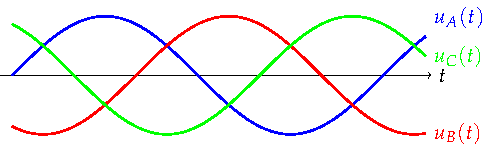
\includegraphics[height=0.3\textheight]{../figs/TensionesTrifasica_ABC.pdf}
\end{center}
\begin{itemize}
\item Secuencia de Fases Inversa (\alert{SFI}): ACB
\end{itemize}
\begin{center}
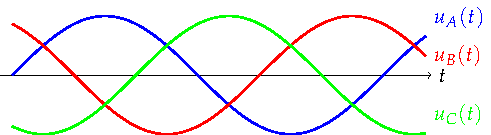
\includegraphics[height=0.3\textheight]{../figs/TensionesTrifasica_ACB.pdf}
\end{center}
\end{frame}

\begin{frame}{Secuencia de fases}{Secuencia de fases directa (SFD)}
\begin{columns}
\begin{column}{0.25\columnwidth}
\begin{center}
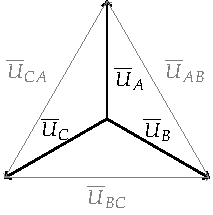
\includegraphics[width=\linewidth]{../figs/FasoresTrifasica_ABC.pdf}
\end{center}
\end{column}
\begin{column}{0.25\columnwidth}
\begin{align*}
  \overline{U}_A &= U_F\phase{{\color{blue}\ang{90}}}\\
  \overline{U}_B &= U_F\phase{\ang{-30}}\\
  \overline{U}_C &= U_F\phase{\ang{-150}}
\end{align*}
\end{column}
\begin{column}{0.5\columnwidth}
	\begin{align*}
		&\overline{U_{AB}}=\overline{U_{A}}-\overline{U_{B}}=\\&=(0+\mathrm{j}\,U_F)-\left(\dfrac{\sqrt{3}\,U_F}{2}-\mathrm{j}\,\dfrac{U_F}{2}\right)=\\
		&=-\dfrac{\sqrt{3}\cdot U_F}{2}+\mathrm{j}\,\dfrac{3\,U_F}{2}=\sqrt{3}\,U_F \phase{ 120^\circ}
	\end{align*}
\end{column}
\end{columns}

\begin{columns}
\begin{column}{0.2\columnwidth}
\begin{align*}
  \overline{U}_A &= U_F\phase{{\ang{90}}}\\
  \overline{U}_B &= U_F\phase{\ang{-30}}\\
  \overline{U}_C &= U_F\phase{\ang{-150}}
\end{align*}
\end{column}
\begin{column}{0.2\columnwidth}
\begin{align*}
  \overline{U}_{AB} &= \sqrt{3}\,U_F\phase{\ang{120}}\\
  \overline{U}_{BC} &= \sqrt{3}\,U_F\phase{\ang{0}}\\
  \overline{U}_{CA} &= \sqrt{3}\,U_F\phase{\ang{-120}}
\end{align*}
\end{column}
\begin{column}{0.4\columnwidth}
\begin{block}{Relación tensión fase-línea SFD}
	\begin{equation*}
		\boxed{
			\begin{array}{l}
				U_L = \sqrt{3}\cdot U_F\\
				\theta_L = \theta_F + 30^\circ\\
			\end{array}
		} 
	\end{equation*}
\end{block}
\end{column}
\end{columns}
\end{frame}


\begin{frame}{Secuencia de fases}{Secuencia de fases inversa (SFI)}
\begin{columns}
\begin{column}{0.25\columnwidth}
\begin{center}
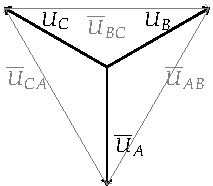
\includegraphics[width=\linewidth]{../figs/FasoresTrifasica_ACB.pdf}
\end{center}
\end{column}
\begin{column}{0.25\columnwidth}
\begin{align*}
  \overline{U}_A &= U_F\phase{{\color{blue}\ang{-90}}}\\
  \overline{U}_B &= U_F\phase{\ang{30}}\\
  \overline{U}_C &= U_F\phase{\ang{150}}
\end{align*}
\end{column}
\begin{column}{0.5\columnwidth}
	\begin{align*}
		&\overline{U_{AB}}=\overline{U_{A}}-\overline{U_{B}}=\\&=(0-\mathrm{j}\,U_F)-\left(\dfrac{\sqrt{3}\,U_F}{2}+\mathrm{j}\,\dfrac{U_F}{2}\right)=\\
		&=-\dfrac{\sqrt{3}\cdot U_F}{2}-\mathrm{j}\,\dfrac{3\,U_F}{2}=\sqrt{3}\,U_F \phase{-120^\circ}
	\end{align*}
\end{column}
\end{columns}

\begin{columns}
\begin{column}{0.2\columnwidth}
\begin{align*}
  \overline{U}_A &= U_F\phase{{\ang{-90}}}\\
  \overline{U}_B &= U_F\phase{\ang{30}}\\
  \overline{U}_C &= U_F\phase{\ang{150}}
\end{align*}
\end{column}
\begin{column}{0.2\columnwidth}
\begin{align*}
  \overline{U}_{AB} &= \sqrt{3}\,U_F\phase{\ang{-120}}\\
  \overline{U}_{BC} &= \sqrt{3}\,U_F\phase{\ang{0}}\\
  \overline{U}_{CA} &= \sqrt{3}\,U_F\phase{\ang{120}}
\end{align*}
\end{column}
\begin{column}{0.4\columnwidth}
\begin{block}{Relación tensión fase-línea SFI}
	\begin{equation*}
		\boxed{
			\begin{array}{l}
				U_L = \sqrt{3}\cdot U_F\\
				\theta_L = \theta_F - 30^\circ\\
			\end{array}
		} 
	\end{equation*}
\end{block}
\end{column}
\end{columns}
\end{frame}

\section{Conexiones en estrella y triángulo}

\subsection{Conexión en estrella}

\begin{frame}{Conexiones en estrella y triángulo}{Conexión en estrella}
\begin{block}{Estrella}
    Se unen los terminales $A'$, $B'$ y $C'$ en un punto común (\alert{neutro}, $N$), quedando libres los terminales $A$, $B$ y $C$:
    \begin{itemize}
        \item Sistema a cuatro hilos
        \item Sistema a tres hilos
    \end{itemize}
\end{block}

\begin{figure}
		\centering
		{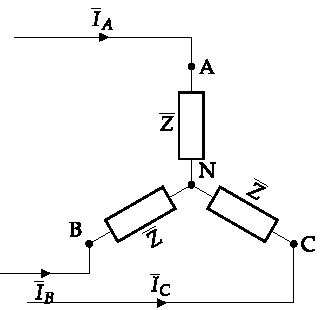
\includegraphics[width=0.25\linewidth]{../figs/EstrellaEquilibrado_Receptor_SN.pdf}}\hfil
		{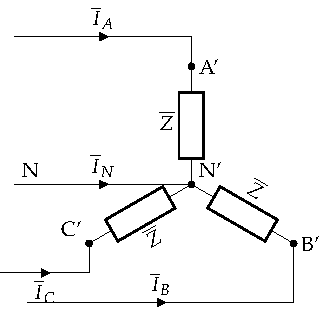
\includegraphics[width=0.25\linewidth]{../figs/EstrellaEquilibrado_Receptor.pdf}}
	\end{figure}
\end{frame}

\begin{frame}{Conexiones en estrella y triángulo}{Receptor en estrella equilibrado}
\begin{columns}
\begin{column}{0.5\columnwidth}
\begin{center}
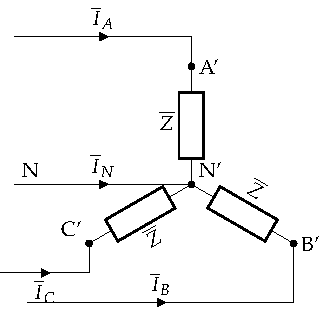
\includegraphics[width=.9\linewidth]{../figs/EstrellaEquilibrado_Receptor.pdf}
\end{center}
\end{column}

\begin{column}{0.5\columnwidth}
\begin{align*}
  \overline{I}_A &= \frac{\overline{U}_A}{\overline{Z}} = \frac{U_F}{Z}\phase{\ang{\pm 90} - \theta} \\
  \overline{I}_B &= \frac{\overline{U}_B}{\overline{Z}} = \frac{U_F}{Z}\phase{\ang{\mp 30} - \theta}\\
  \overline{I}_C &= \frac{\overline{U}_C}{\overline{Z}} = \frac{U_F}{Z}\phase{\ang{\mp 150} - \theta}
\end{align*}

\[
  \overline{I}_A  + \overline{I}_B + \overline{I}_C + \overline{I}_N = 0 \rightarrow \boxed{\overline{I}_N = 0}
\]

Corriente de Fase (\alert{igual a la de línea}):

\[
  \boxed{I_F={I}_A = {I}_B = {I}_C = \frac{U_F}{Z}}
\]

\end{column}
\end{columns}
\end{frame}

\begin{frame}{Conexiones en estrella y triángulo}{Receptor en estrella equilibrado --- Ejemplo}
    \textbf{Un sistema a cuatro hilos y SFI alimenta tres impedancias $\overline{Z}=10\phase{60^\circ}\;\Omega$, conectadas en estrella a la tensión $200\,\sqrt{3}$ V. Determinar las corrientes de línea y el diagrama fasorial.}
\end{frame}

\subsection{Conexión en triángulo}

\begin{frame}{Conexiones en estrella y triángulo}{Conexión en triángulo} 
\begin{block}{Triángulo}
    Se conecta el terminal de polaridad negativa de una fase, con el de referencia positiva de otra fase ($A'$ con $B$, $B'$ con $C$ y $C'$ con $A$):
    \begin{itemize}
        \item Sistema a tres hilos
    \end{itemize}
\end{block}

\begin{figure}
		\centering
		{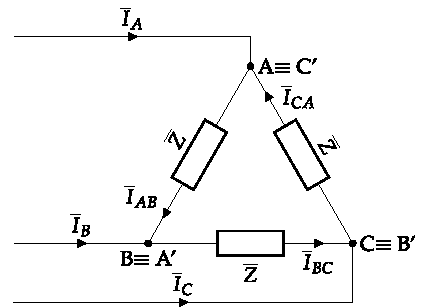
\includegraphics[width=0.35\linewidth]{../figs/TrianguloEquilibrado_Receptor.pdf}}
	\end{figure}
\end{frame}

\begin{frame}{Conexiones en estrella y triángulo}{Receptor en triángulo equilibrado}
\begin{columns}
\begin{column}{0.5\columnwidth}
\begin{center}
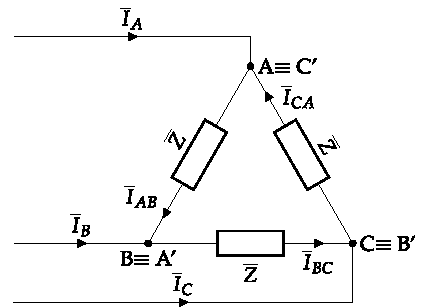
\includegraphics[width=.9\linewidth]{../figs/TrianguloEquilibrado_Receptor.pdf}
\end{center}
\end{column}

\begin{column}{0.5\columnwidth}
\begin{align*}
  \overline{I}_{AB} &= \frac{\overline{U}_{AB}}{\overline{Z}} = \frac{U_F}{Z}\phase{\ang{\pm 120} - \theta} \\
  \overline{I}_{BC} &= \frac{\overline{U}_{BC}}{\overline{Z}} = \frac{U_F}{Z}\phase{0 - \theta}\\
  \overline{I}_{CA} &= \frac{\overline{U}_{CA}}{\overline{Z}} = \frac{U_F}{Z}\phase{\ang{\mp 120} - \theta}
\end{align*}

\[
   \overline{I}_{AB}  + \overline{I}_{BC} + \overline{I}_{CA}  = 0 
\]

Corriente de Fase:
\[
  \boxed{I_F = {I}_{AB} = {I}_{BC} = {I}_{CA} = \frac{U_F}{Z}}
\]
\end{column}
\end{columns}
\end{frame}


\begin{frame}{Conexiones en estrella y triángulo}{Receptor en triángulo equilibrado}
\begin{columns}
\begin{column}{0.5\columnwidth}
\begin{center}
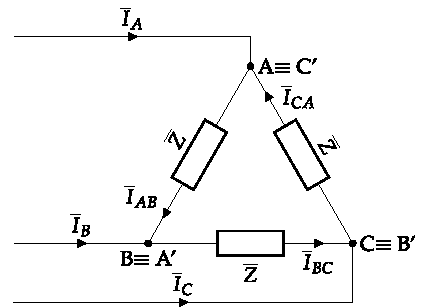
\includegraphics[width=.9\linewidth]{../figs/TrianguloEquilibrado_Receptor.pdf}
\end{center}
\end{column}

\begin{column}{0.5\columnwidth}
\begin{align*}
  \overline{I}_A &= \overline{I}_{AB} - \overline{I}_{CA} = \sqrt{3} \cdot \frac{U}{Z}\phase{\ang{\pm 90} - \theta}\\
  \overline{I}_B &= \overline{I}_{BC} - \overline{I}_{AB} = \sqrt{3} \cdot \frac{U}{Z}\phase{\ang{\mp 30} - \theta}\\
  \overline{I}_C &= \overline{I}_{CA} - \overline{I}_{BC} = \sqrt{3} \cdot \frac{U}{Z}\phase{\ang{\mp 150} - \theta}\\
\end{align*}

Corriente de Línea:
\[
  \boxed{I_L = {I}_A = {I}_B = {I}_C = \sqrt{3} \cdot \frac{U_F}{Z}}
\]

\[
  \boxed{I = \sqrt{3} \cdot I_F}
\]
\end{column}
\end{columns}
\end{frame}

\begin{frame}{Conexiones en estrella y triángulo}{Receptor en triángulo equilibrado --- Ejemplo}

\textbf{Un sistema trifásico de secuencia directa y tensión $200$ V alimenta tres impedancias iguales $\overline{Z}=10\phase{30^\circ}\;\Omega$ conectadas en triángulo. Determinar las corrientes de fase y línea y dibujar el diagrama fasorial.}
    
\end{frame}

\section{Potencia en sistemas trifásicos}

\begin{frame}{Potencia en sistemas trifásicos}{Potencia instantánea}
Supongamos un receptor equilibrado en estrella con SFD:

\begin{columns}
\begin{column}{0.5\columnwidth}
\begin{align*}
  u_A(t) &= \sqrt{2} U_F \cos(\omega t + \ang{90})\\
  u_B(t) &= \sqrt{2} U_F \cos(\omega t - \ang{30})\\
  u_C(t) &= \sqrt{2} U_F \cos(\omega t - \ang{150})
\end{align*}

\begin{align*}
  i_A(t) &= \sqrt{2} I_F \cos(\omega t + \ang{90} - \theta)\\
  i_B(t) &= \sqrt{2} I_F \cos(\omega t - \ang{30} - \theta)\\
  i_C(t) &= \sqrt{2} I_F \cos(\omega t - \ang{150} - \theta)
\end{align*}
\end{column}

\begin{column}{0.5\columnwidth}
\begin{align*}
  p_A(t) &= u_A(t) \cdot i_A(t)\\
  p_B(t) &= u_C(t) \cdot i_B(t)\\
  p_C(t) &= u_C(t) \cdot i_C(t)\\
  \\
  p(t) &= p_A(t) + p_B(t) + p_C(t)
\end{align*}
\end{column}
\end{columns}
\end{frame}

\begin{frame}{Potencia en sistemas trifásicos}{Potencia instantánea}
\begin{align*}
  p(t) &= \sqrt{2}U_F  \cos(\omega t + \ang{90}) \cdot \sqrt{2}I_F\cos(\omega t + \ang{90} - \theta) +\\
       &+ \sqrt{2}U_F \cos(\omega t - \ang{30}) \cdot \sqrt{2}I_F \cos(\omega t - \ang{30} - \theta) +\\
       &+ \sqrt{2}U_F \cos(\omega t - \ang{150}) \cdot \sqrt{2}I_F \cos(\omega t - \ang{150} - \theta)
\end{align*}
\[
  \cos(\alpha) \cdot \cos(\beta) = \frac{1}{2} \cdot (\cos(\alpha + \beta) + \cos(\alpha - \beta))
\]
\begin{align*}
  p(t) &= U_F I_F [{\color{gray}\cos(2 \omega t + \ang{180} -\theta)} + \cos(\theta)] +\\
       &+ U_F I_F [{\color{gray}\cos(2 \omega t - \ang{60} - \theta)} + \cos(\theta)] +\\
       &+ U_F I_F [{\color{gray}\cos(2 \omega t - \ang{300} - \theta)} + \cos(\theta)]
\end{align*}
\[
  \boxed{p(t) = 3 \cdot U_F \cdot I_F \cdot \cos (\theta) }
\]
\end{frame}

\begin{frame}{Potencia en sistemas trifásicos}{Receptor en estrella equilibrado}
\begin{columns}
\begin{column}{0.4\columnwidth}
\begin{center}
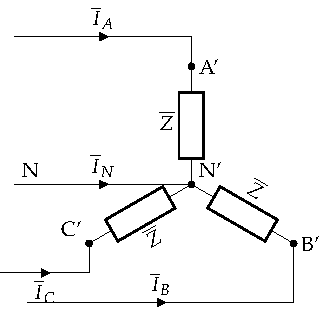
\includegraphics[width=.9\linewidth]{../figs/EstrellaEquilibrado_Receptor.pdf}
\end{center}
\end{column}

\begin{column}{0.6\columnwidth}
\begin{align*}
P_F &= U_F\cdot I_F\cdot\cos(\theta)\\
  P_T &= 3 \cdot P_F= 3 \cdot U_F\cdot I_F \cdot\cos(\theta)
\end{align*}

\begin{align*}
  I_F &= I_L\\
  U_F &= \frac{U_L}{\sqrt{3}}
\end{align*}

\begin{align*}
  P_T &= 3\cdot U_F \cdot I_F \cos(\theta) = \sqrt{3}\cdot  U_L \cdot I_L\cdot \cos(\theta)\\
  Q_T &= 3\cdot U_F \cdot I_F \sin(\theta) = \sqrt{3}\cdot  U_L \cdot I_L\cdot \sin(\theta)\\
  S_T &= \sqrt{P_T^2 + Q_T^2} = 3\cdot U_F\cdot I_F = \sqrt{3}\cdot U_L\cdot I_L
\end{align*}
\end{column}
\end{columns}
\end{frame}


\begin{frame}{Potencia en sistemas trifásicos}{Receptor en triángulo equilibrado}
\begin{columns}
\begin{column}{0.4\columnwidth}
\begin{center}
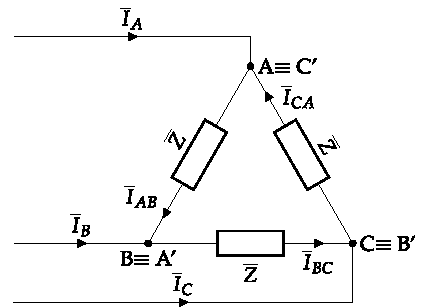
\includegraphics[width=.9\linewidth]{../figs/TrianguloEquilibrado_Receptor.pdf}
\end{center}
\end{column}

\begin{column}{0.6\columnwidth}
\begin{align*}
P_F &= U_F\cdot I_F\cdot\cos(\theta)\\
  P_T &= 3 \cdot P_F= 3 \cdot U_F\cdot I_F \cdot\cos(\theta)
\end{align*}

\begin{align*}
  I_F &= \frac{I_L}{\sqrt{3}}\\
  U_F &= {U_L}
\end{align*}

\begin{align*}
  P_T &= 3\cdot U_F \cdot I_F \cos(\theta) = \sqrt{3}\cdot  U_L \cdot I_L\cdot \cos(\theta)\\
  Q_T &= 3\cdot U_F \cdot I_F \sin(\theta) = \sqrt{3}\cdot  U_L \cdot I_L\cdot \sin(\theta)\\
  S_T &= \sqrt{P_T^2 + Q_T^2} = 3\cdot U_F\cdot I_F = \sqrt{3}\cdot U_L\cdot I_L
\end{align*}
\end{column}
\end{columns}
\end{frame}

\begin{frame}{Potencia en sistemas trifásicos}{Ejemplo}
    \textbf{Una red trifásica de $20$ kV de tensión de línea alimenta a una instalación que dispone de dos cargas:
\begin{itemize}
    \item Carga 1: conexión triángulo, potencia nominal aparente de $300$ kVA y fdp $0.85$ inductivo
    \item Carga 2: conexión estrella, potencia nominal aparente de $100$ kVA y fdp $0.95$ capacitivo
\end{itemize}
Se pide calcular las potencias totales $P$, $Q$ y $S$, el módulo de la corriente de línea absorbida y el factor de potencia del conjunto.}
\end{frame}

% \begin{frame}{Comparativa Monofásica-Trifásica}
% Comparemos un sistema monofásico y un sistema trifásico (3H) que transmiten la \alert{misma potencia activa} y funcionan a la \alert{misma tensión entre líneas}.
% \[
% U I_1 \cos\theta = P_1 = P_3 = \sqrt{3}U I_3 \cos\theta \rightarrow \boxed{I_1 = \sqrt{3} I_3}
% \]
% Las \alert{pérdidas en la línea} deben ser \alert{iguales} para salvar la \alert{misma distancia}:
% \[
%   2R_1I_1^2 = P_{1l} = P_{3l} = 3R_3I_3^2
% \]
% Sustituyendo la relación de corrientes y teniendo en cuenta la relación entre resistencia y sección:
% \[
%   2\cdot R_1 \cdot 3I_3^2 = 3\cdot R_3 I_3^2 \rightarrow R_1 = \frac{1}{2} R_3 \rightarrow \boxed{S_1 = 2 \cdot S_3}
% \]

% Finalmente, la relación entre masas de conductor es:

% \[
%   \frac{m_3}{m_1} = \frac{3 \cdot S_3}{2 \cdot S_1} = \boxed{\frac{3}{4}}
% \]
% \end{frame}

\section{Medida de potencia en sistemas trifásicos}

\begin{frame}{Medida de potencia en sistemas trifásicos}{Recordatorio: vatímetro}
\begin{center}
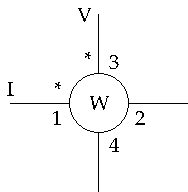
\includegraphics[height=0.5\textheight]{../figs/vatimetro_2.pdf}
\end{center}

\alert{Vatímetro}: equipo de medida de 4 terminales (1 par para tensión, 1 par para corriente):

\begin{equation*}
	    W=\overline{I_{1,2}}\,\circ\,\overline{U_{3,4}}=I_{1,2}\cdot U_{3,4}\cdot \widehat{(I_{1,2}, U_{3,4})}
	\end{equation*}
\end{frame}

\subsection{Sistemas a cuatro hilos}
\begin{frame}{Medida de potencia en sistemas trifásicos}{Sistema a cuatro hilos --- caso general}
\begin{columns}
\begin{column}{0.7\columnwidth}
\begin{center}
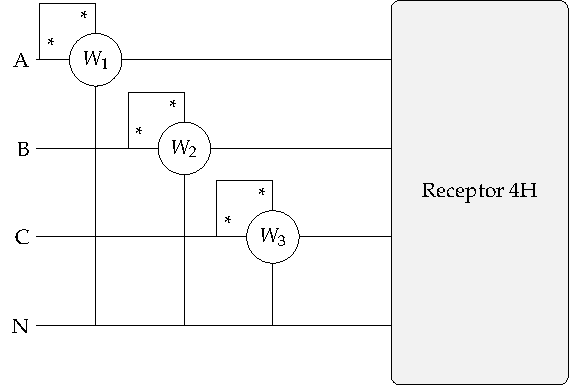
\includegraphics[height=0.75\textheight]{../figs/Potencia4H.pdf}
\end{center}
\end{column}

\begin{column}{0.3\columnwidth}
\begin{align*}
  W_1 &= \Re(\overline{U}_A \cdot \overline{I}_A^*) = P_A\\
  W_2 &= \Re(\overline{U}_B \cdot \overline{I}_B^*) = P_B\\
  W_3 &= \Re(\overline{U}_C \cdot \overline{I}_C^*) = P_C\\
\end{align*}

\[
  \boxed{P = W_1 + W_2 + W_3}
\]
\end{column}
\end{columns}
\end{frame}


\begin{frame}{Medida de potencia en sistemas trifásicos}{Sistema a cuatro hilos equilibrado}
\begin{columns}
\begin{column}{0.7\columnwidth}
\begin{center}
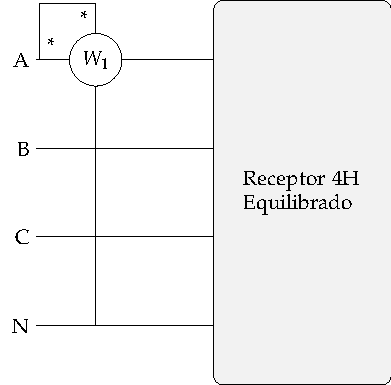
\includegraphics[height=0.75\textheight]{../figs/Potencia4H_Equilibrado.pdf}
\end{center}
\end{column}

\begin{column}{0.4\columnwidth}
\[
  P_A = P_B = P_C
\]

\[
\boxed{P = 3 \cdot W_1}
\]
\end{column}
\end{columns}
\end{frame}

\subsection{Sistemas a tres hilos}

\begin{frame}{Medida de potencia en sistemas trifásicos}{Sistema a tres hilos --- Estrella}
\begin{equation*}
	    P_T=P_A+P_B+P_C
	\end{equation*}
	\begin{columns}
	\begin{column}{0.6\linewidth}
Teniendo en cuenta que debe cumplirse la 1LK en $N$:
	\begin{equation*}
	    \overline{I_A}+\overline{I_B}+\overline{I_C}\Rightarrow \overline{I_C}=-(\overline{I_A}+\overline{I_B})
	\end{equation*}
	y, sustituyendo en la potencia total: 
	\begin{align*}
	    P_T&=P_A+P_B+P_C=\overline{U_{A}}\;\circ\; \overline{I_A} + \overline{U_{B}}\;\circ\; \overline{I_B} + \overline{U_{C}}\;\circ\,\overline{I_C}=\\
	    &=\overline{U_{A}}\;\circ\; \overline{I_A}+\overline{U_{B}}\;\circ\; \overline{I_B}+\overline{U_{C}}\;\circ\left(-(\overline{I_A}+\overline{I_B})\right)=\nonumber \\
	    & =(\overline{U_A}-\overline{U_C})\;\circ\; \overline{I_A}+(\overline{U_B}-\overline{U_C})\;\circ\; \overline{I_B}\Rightarrow \\
	    &\Rightarrow \boxed{P_T=\overline{U_{\textcolor{red}{A}C}}\,\circ\,\overline{I_{\textcolor{red}{A}}}+\overline{U_{\textcolor{cyan}{B}C}}\,\circ\,\overline{I_{\textcolor{cyan}{B}}}}
	\end{align*}
	\end{column}
	\begin{column}{0.4\linewidth}
	\begin{center}
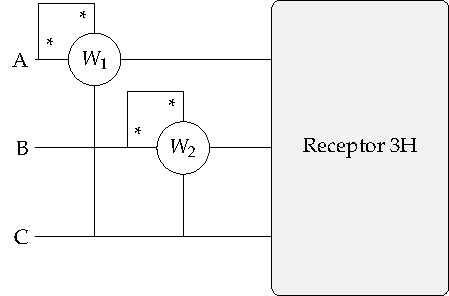
\includegraphics[width=\linewidth]{../figs/Potencia3H.pdf}
\end{center}
	\end{column}
	\end{columns}
	
\end{frame}

\begin{frame}{Medida de potencia en sistemas trifásicos}{Sistema a tres hilos --- Triángulo}
	\begin{align*}
	    P_{AB}=U_{AB}\cdot I_{AB} \cdot \cos(\theta_{AB});\qquad 
	    &P_{BC}=U_{BC}\cdot I_{BC} \cdot \cos(\theta_{BC});\qquad 
	    P_{CA}=U_{CA}\cdot I_{CA} \cdot \cos(\theta_{CA})\\
	    &P_T=P_{AB}+P_{BC}+P_{CA}
	\end{align*}
	Teniendo en cuenta que debe cumplirse la 1LK en los nudos $A$ y $B$:
	\begin{align*}
	    \overline{I_A}=\overline{I_{AB}}-\overline{I_{CA}}\Rightarrow \overline{I_{CA}}=\overline{I_{AB}}-\overline{I_A}\\
	    \overline{I_B}=\overline{I_{BC}}-\overline{I_{AB}}\Rightarrow \overline{I_{BC}}=\overline{I_{B}}+\overline{I_{AB}}
	\end{align*}
	y, sustituyendo en la potencia total:
		\begin{align*}
	    P_T&=P_{AB}+P_{BC}+P_{CA}=\overline{U_{AB}}\;\circ\; \overline{I_{AB}} + \overline{U_{BC}}\;\circ\;\left(\overline{I_B}+\overline{I_{AB}} \right)  + \overline{U_{CA}}\;\circ\,(\overline{I_{AB}}-\overline{I_A})=\nonumber \\
	    & =\underbrace{(\overline{U_{AB}}+\overline{U_{BC}}+\overline{U_{CA}})}_{0}\;\circ\; \overline{I_{AB}}+\overline{U_{BC}}\,\circ\,\overline{I_B}\underbrace{-\overline{U_{CA}}}_{\overline{U_{AC}}}\;\circ\; \overline{I_A}\Rightarrow \boxed{P_T=\overline{U_{\textcolor{red}{A}C}}\,\circ\,\overline{I_{\textcolor{red}{A}}}+\overline{U_{\textcolor{cyan}{B}C}}\,\circ\,\overline{I_{\textcolor{cyan}{B}}}}
	\end{align*}
\end{frame}

\subsection{Método de los dos vatímetros}

\begin{frame}{Medida de potencia en sistemas trifásicos}{Método de los dos vatímetros}
Se eligen \alert{dos líneas cualesquiera} a las que se conectan las \alert{bobinas de intensidad} del vatímetro. Las \alert{entradas de las bobinas de tensión} se conectan a las \alert{mismas líneas} que las de intensidad y, las \alert{salidas}, a la \alert{línea no usada}. Si alguno de los vatímetros da una lectura negativa, en la suma se considerará con el signo $-$.  
\begin{columns}
\begin{column}{0.6\linewidth}
\begin{figure}[H]
	    \centering
	    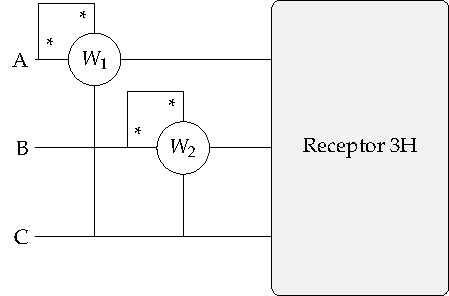
\includegraphics{../figs/Potencia3H.pdf}
	\end{figure}
\end{column}
\begin{column}{0.4\linewidth}
\begin{equation*}
    P_T=W_1+W_2
\end{equation*}
\end{column}
\end{columns}
\end{frame}

\begin{frame}{Medida de potencia en sistemas trifásicos}{Método de los dos vatímetros --- SFD}
Supóngase un receptor en estrella de carácter inductivo con vatímetros en $A$ y $B$:
\begin{columns}
\begin{column}{0.38\columnwidth}
	    \centering
	    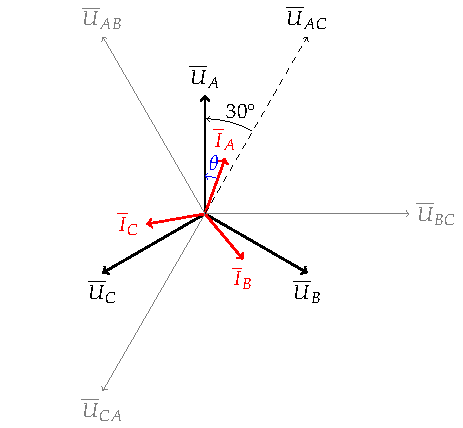
\includegraphics[width=0.9\linewidth]{../figs/fasores_potencia3H.pdf}
	    \begin{align*}
	    W_1&=\overline{U_{AC}}\,\circ\,\overline{I_A}\\ 
	    W_2&=\overline{U_{BC}}\,\circ\,\overline{I_B}
	\end{align*}
\end{column}
\pause
\begin{column}{0.3\columnwidth}
	Se sabe que:
	\begin{align*}
	   &\overline{U_{AC}}=-\overline{U_{CA}}=\\
	   &=U_L\phase{-120^\circ-180^\circ}=\\
	   &=U_L\phase{60^\circ}\\ &\overline{U_{BC}}=U_L\phase{0^\circ}\\ &\overline{I_A}=I_L\phase{90^\circ-\theta}\\ &\overline{I_B}=I_L\phase{-30^\circ-\theta} 
	\end{align*}
\end{column}
\pause
\begin{column}{0.3\linewidth}
Por tanto: 
	\begin{align*}
	    W_1&=U_L\;I_L\;\cos{(\theta-30^\circ)}\\ W_2&={U_L}\; {I_L}\;\cos{(\theta+30^\circ)}
	\end{align*}
\end{column}
\end{columns}
\end{frame}

\begin{frame}{Medida de potencia en sistemas trifásicos}{Método de los dos vatímetros --- SFD}
\begin{columns}
\begin{column}{0.38\columnwidth}
	    \centering
	    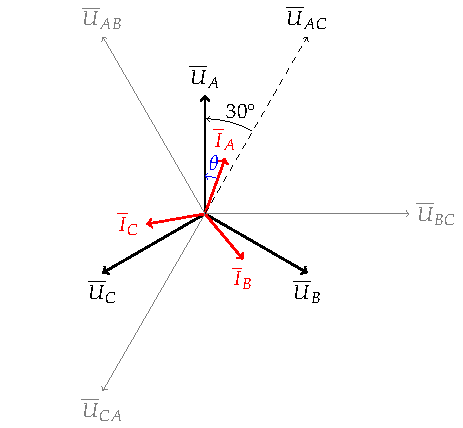
\includegraphics[width=0.9\linewidth]{../figs/fasores_potencia3H.pdf}
	    \begin{align*}
	    W_1&=\overline{U_{AC}}\,\circ\,\overline{I_A}\\ 
	    W_2&=\overline{U_{BC}}\,\circ\,\overline{I_B}
	\end{align*}
\end{column}
\begin{column}{0.6\columnwidth}
Desarrollando los cosenos:
\begin{align*}
  \cos(\theta-{30^\circ}) &= \cos(\theta)\,\cos({30^\circ}) + \sin(\theta)\,\sin({30^\circ})\\
  \cos(\theta+{30^\circ}) &= \cos(\theta)\,\cos({30^\circ}) - \sin(\theta)\,\sin({30^\circ})
\end{align*}
Si se suman las medidas de los dos vatímetros:
\begin{align*}
     \boxed{W_1 + W_2 = \sqrt{3}\,U_L\, I_L\,\cos(\theta) = P_T}
\end{align*}
Si se restan las medidas de los dos vatímetros:
\begin{align*}
    \boxed{W_1 - W_2 = U_L\, I_L\,\sin(\theta) = \dfrac{Q_T}{\sqrt{3}}}
\end{align*}
\end{column}
\end{columns}
\end{frame}

\begin{frame}{Medida de potencia en sistemas trifásicos}{Método de los dos vatímetros --- SFD --- Otras conexiones}
\[
  \boxed{(ABC): A \triangleright B \triangleright C \Longrightarrow \{AB, BC, CA\}}
\]
\begin{align*}
  P = W_1 + W_2\qquad \qquad Q = \sqrt{3}(W_1 - W_2)
\end{align*}
\begin{columns}
\begin{column}{0.33\columnwidth}
\begin{center}
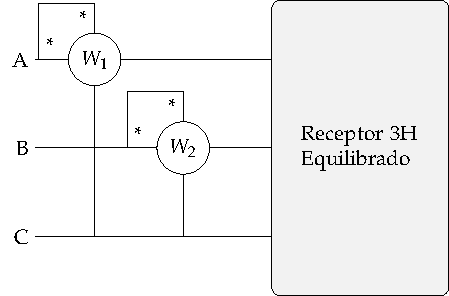
\includegraphics[width=.8\linewidth]{../figs/Potencia_3H_equilibrado_AB.pdf}
\end{center}
\begin{align*}
  W_1&: AC \notin SFD\\
  W_2&: BC \in SFD
\end{align*}
\end{column}
\begin{column}{0.33\columnwidth}
\begin{center}
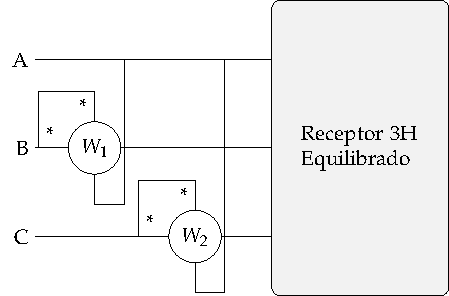
\includegraphics[width=.8\linewidth]{../figs/Potencia_3H_equilibrado_BC.pdf}
\end{center}
\begin{align*}
  W_1&: BA \notin SFD\\
  W_2&: CA \in SFD
\end{align*}
\end{column}

\begin{column}{0.33\columnwidth}
\begin{center}
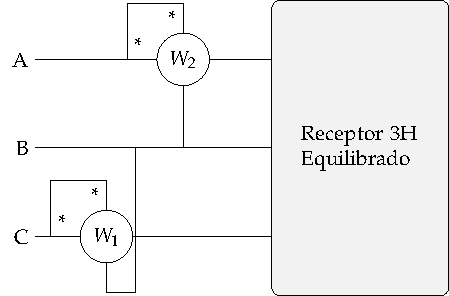
\includegraphics[width=.8\linewidth]{../figs/Potencia_3H_equilibrado_CA.pdf}
\end{center}
\begin{align*}
  W_1&: CB \notin SFD\\
  W_2&: AB \in SFD
\end{align*}
\end{column}
\end{columns}
\end{frame}

\begin{frame}{Medida de potencia en sistemas trifásicos}{Método de los dos vatímetros --- SFI}
Supóngase un receptor en estrella de carácter inductivo con vatímetros en $B$ y $A$:
\begin{columns}
\begin{column}{0.38\columnwidth}
	    \centering
	    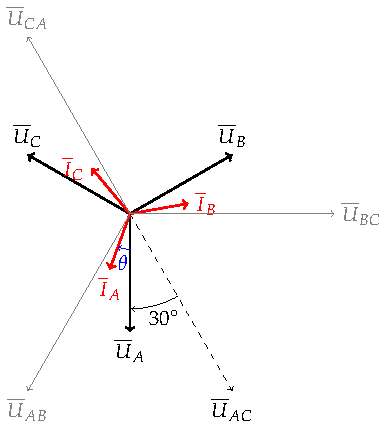
\includegraphics[width=0.8\linewidth]{../figs/fasores_potencia3H_SFI.pdf}
	    \begin{align*}
	    W_1&=\overline{U_{BC}}\,\circ\,\overline{I_B}\\ 
	    W_2&=\overline{U_{AC}}\,\circ\,\overline{I_A}
	\end{align*}
\end{column}
\pause
\begin{column}{0.3\columnwidth}
	Se sabe que:
	\begin{align*}
	    &\overline{U_{BC}}=U_L\phase{0^\circ}\\
	   &\overline{U_{AC}}=-\overline{U_{CA}}=\\
	   &=U_L\phase{120^\circ+180^\circ}=\\
	   &=U_L\phase{-60^\circ}\\ &\overline{I_B}=I_L\phase{30^\circ-\theta} \\  &\overline{I_A}=I_L\phase{-90^\circ-\theta}
	\end{align*}
\end{column}
\pause
\begin{column}{0.3\linewidth}
Por tanto: 
	\begin{align*}
	    W_1&=U_L\;I_L\;\cos{(\theta-30^\circ)}\\ W_2&={U_L}\; {I_L}\;\cos{(\theta+30^\circ)}
	\end{align*}
	\alert{Idénticos a SFD}
\end{column}
\end{columns}
\end{frame}

\begin{frame}{Medida de potencia en sistemas trifásicos}{Método de los dos vatímetros --- SFI}
\begin{columns}
\begin{column}{0.38\columnwidth}
	    \centering
	    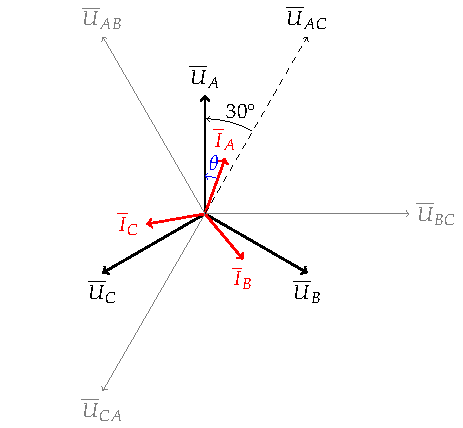
\includegraphics[width=0.8\linewidth]{../figs/fasores_potencia3H.pdf}
	    \begin{align*}
	    W_1&=\overline{U_{BC}}\,\circ\,\overline{I_B}\\ 
	    W_2&=\overline{U_{AC}}\,\circ\,\overline{I_A}
	\end{align*}
\end{column}
\begin{column}{0.6\columnwidth}
Desarrollando los cosenos:
\begin{align*}
  \cos(\theta-{30^\circ}) &= \cos(\theta)\,\cos({30^\circ}) + \sin(\theta)\,\sin({30^\circ})\\
  \cos(\theta+{30^\circ}) &= \cos(\theta)\,\cos({30^\circ}) - \sin(\theta)\,\sin({30^\circ})
\end{align*}
Si se suman las medidas de los dos vatímetros:
\begin{align*}
     \boxed{W_1 + W_2 = \sqrt{3}\,U_L\, I_L\,\cos(\theta) = P_T}
\end{align*}
Si se restan las medidas de los dos vatímetros:
\begin{align*}
    \boxed{W_1 - W_2 = U_L\, I_L\,\sin(\theta) = \dfrac{Q_T}{\sqrt{3}}}
\end{align*}
\end{column}
\end{columns}
\end{frame}

\begin{frame}{Medida de potencia en sistemas trifásicos}{Método de los dos vatímetros --- SFI --- Otras conexiones}
\[
  \boxed{(ACB): A \triangleright C \triangleright B \Longrightarrow \{AC, CB, BA\}}
\]
\begin{align*}
  P = W_1 + W_2\qquad \qquad Q = \sqrt{3}(W_1 - W_2)
\end{align*}
\begin{columns}
\begin{column}{0.33\columnwidth}
\begin{center}
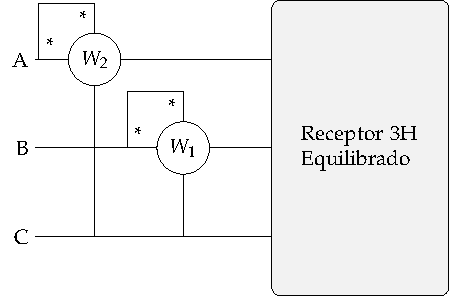
\includegraphics[width=.8\linewidth]{../figs/Potencia3H_Equilibrado_AB_SFI.pdf}
\end{center}
\begin{align*}
  W_1&: BC \notin SFI\\
  W_2&: AC \in SFI\\
\end{align*}
\end{column}
\begin{column}{0.33\columnwidth}
\begin{center}
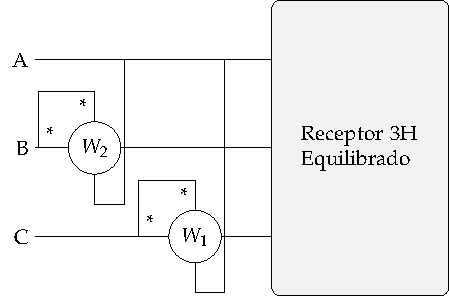
\includegraphics[width=.8\linewidth]{../figs/Potencia3H_Equilibrado_BC_SFI.pdf}
\end{center}
\begin{align*}
  W_1&: CA \notin SFI\\
  W_2&: BA \in SFI\\
\end{align*}
\end{column}

\begin{column}{0.33\columnwidth}
\begin{center}
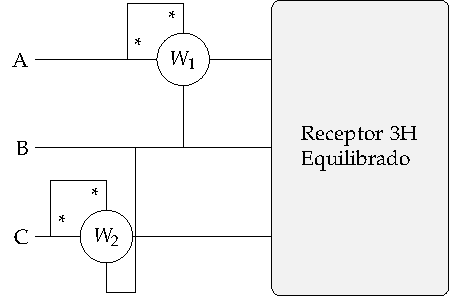
\includegraphics[width=.8\linewidth]{../figs/Potencia3H_Equilibrado_CA_SFI.pdf}
\end{center}
\begin{align*}
  W_1&: AB \notin SFI\\
  W_2&: CB \in SFI\\
\end{align*}
\end{column}
\end{columns}
\end{frame}

\begin{frame}{Medida de potencia en sistemas trifásicos}{Método de los dos vatímetros --- Ejemplo}
    \textbf{Hallar la indicación del voltímetro en el sistema trifásico equilibrado de SFD de la figura, sabiendo que: $W_1=700$ W; $W_2=400$ W; $\overline{Z_L}=1+\mathrm{j}2\Omega$; $\overline{Z_1}=100\Omega$; $\overline{Z_2}=47\phase{37^\circ}\Omega$.}
\begin{figure}[H]
    \centering
    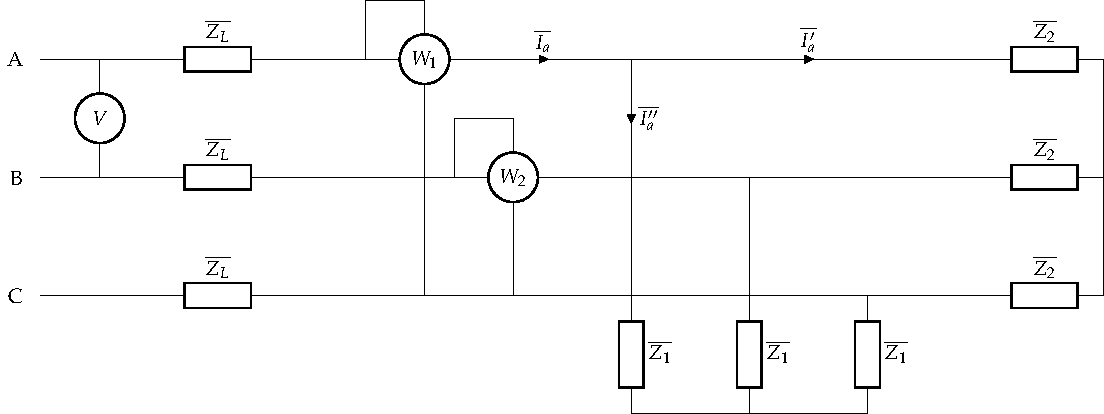
\includegraphics[width=0.8\linewidth]{../figs/ej_dosvat.pdf}
\end{figure}
\end{frame}

\subsection{Medida de potencia reactiva con un vatímetro}

\begin{frame}{Medida de potencia en sistemas trifásicos}{Medida de reactiva con un vatímetro}
Supóngase un receptor en estrella de carácter inductivo y SFD:

\begin{columns}
\begin{column}{0.38\columnwidth}
	    \centering
	    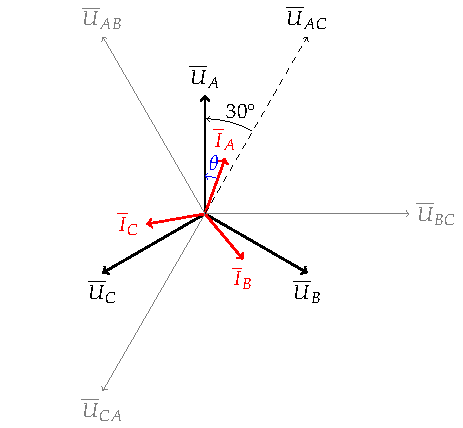
\includegraphics[width=0.9\linewidth]{../figs/fasores_potencia3H.pdf}
	    \begin{align*}
	    W&=\overline{U_{BC}}\,\circ\,\overline{I_A}
	\end{align*}
\end{column}
\pause
\begin{column}{0.3\columnwidth}
	Se sabe que:
	\begin{align*}
  &\overline{U}_{BC} = U_L\phase{0}\\
  &\overline{I}_A = I_L\phase{\ang{90} - \theta}
\end{align*}
Por tanto: 
	\begin{align*}
	     W&=U_L\cdot I_L \cdot\cos(\theta-\ang{90})=\\
	     &= U_L\cdot I_L \cdot \sin(\theta)\Rightarrow\\
	     &\Rightarrow\boxed{W = \frac{Q_T}{\sqrt{3}}}
	\end{align*}
\end{column}
\pause
\begin{column}{0.3\linewidth}
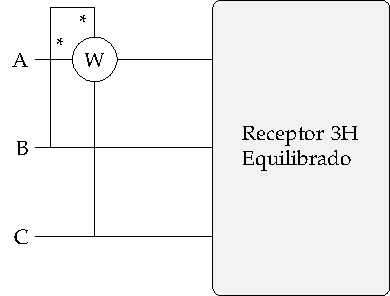
\includegraphics[width=.9\linewidth]{../figs/Reactiva3H_A-BC.pdf}
\end{column}
\end{columns}
\end{frame}

\begin{frame}{Medida de potencia en sistemas trifásicos}{Medida de reactiva con un vatímetro --- Otras conexiones}
\begin{columns}
\begin{column}{0.33\columnwidth}
\begin{center}
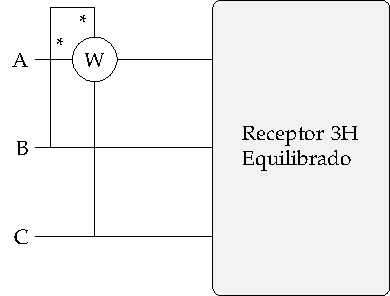
\includegraphics[height=0.25\textheight]{../figs/Reactiva3H_A-BC.pdf}
\end{center}
\begin{align*}
  BC &\in SFD\\
  BC &\notin SFI
\end{align*}
\end{column}
\begin{column}{0.33\columnwidth}
\begin{center}
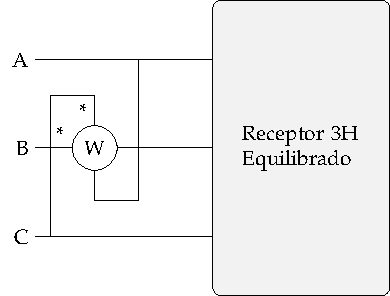
\includegraphics[height=0.25\textheight]{../figs/Reactiva3H_B-CA.pdf}
\end{center}
\begin{align*}
  CA &\in SFD\\
  CA &\notin SFI
\end{align*}
\end{column}
\begin{column}{0.33\columnwidth}
\begin{center}
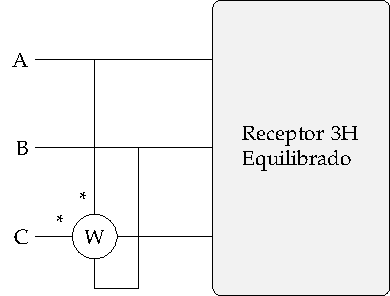
\includegraphics[height=0.25\textheight]{../figs/Reactiva3H_C-AB.pdf}
\end{center}
\begin{align*}
  AB &\in SFD\\
  AB &\notin SFI
\end{align*}
\end{column}
\end{columns}
\begin{align*}
SFD &\rightarrow \boxed{W = \frac{Q_T}{\sqrt{3}}}\\
SFI &\rightarrow \boxed{W =  - \frac{Q_T}{\sqrt{3}}}
\end{align*}
\end{frame}

\begin{frame}{Medida de potencia en sistemas trifásicos}{Medida de reactiva con un vatímetro --- Otras conexiones}
\begin{columns}
\begin{column}{0.33\columnwidth}
\begin{center}
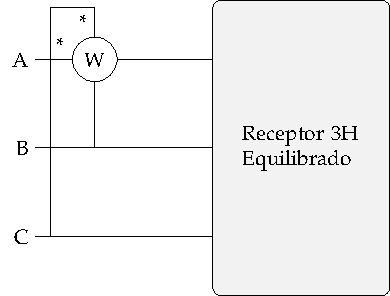
\includegraphics[height=0.25\textheight]{../figs/Reactiva3H_A-CB.pdf}
\end{center}
\begin{align*}
  CB &\notin SFD\\
  CB &\in SFI
\end{align*}
\end{column}
\begin{column}{0.33\columnwidth}
\begin{center}
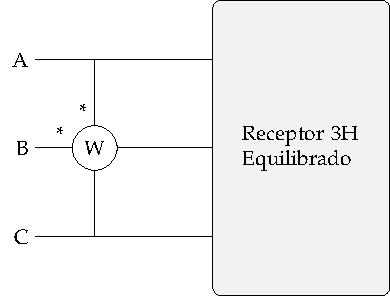
\includegraphics[height=0.25\textheight]{../figs/Reactiva3H_B-AC.pdf}
\end{center}
\begin{align*}
  AC &\notin SFD\\
  AC &\in SFI
\end{align*}
\end{column}
\begin{column}{0.33\columnwidth}
\begin{center}
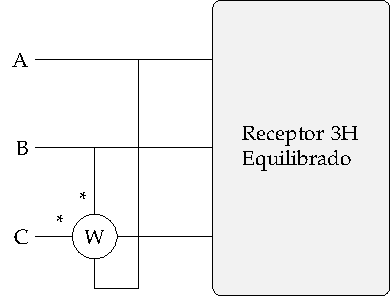
\includegraphics[height=0.25\textheight]{../figs/Reactiva3H_C-BA.pdf}
\end{center}
\begin{align*}
  BA &\notin SFD\\
  BA &\in SFI
\end{align*}
\end{column}
\end{columns}
\begin{align*}
SFD &\rightarrow \boxed{W = - \frac{Q_T}{\sqrt{3}}}\\
SFI &\rightarrow \boxed{W = \frac{Q_T}{\sqrt{3}}}
\end{align*}
\end{frame}

\begin{frame}{Medida de potencia en sistemas trifásicos}{Medida de reactiva con un vatímetro}
    \textbf{El sistema trifásico de la figura es de 380 V, 50 Hz. Sabiendo que la carga es equilibrada y consume 24 kW con un factor de potencia de 0,8 (inductivo), que las tensiones de línea son equilibradas y que se tiene una SFD, se pide calcular:
\begin{itemize}
    \item Valor de las intensidades de línea en forma fasorial
    \item Lectura de los vatímetros
\end{itemize}}
\begin{figure}[H]
    \centering
    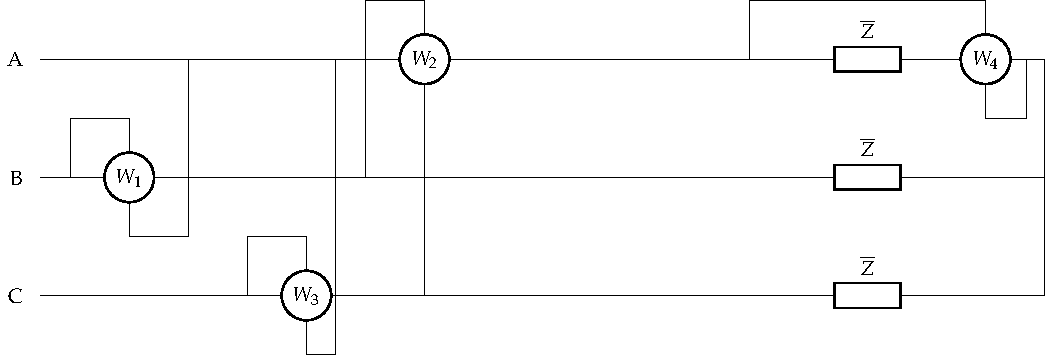
\includegraphics[width=.7\linewidth]{../figs/Q_vat.pdf}
\end{figure}
\end{frame}

\section{Mejora del factor de potencia}

\begin{frame}{Mejora del factor de potencia}
    \begin{itemize}
\item En trifásica existen dos posibilidades:
\begin{itemize}
\item Conexión en triángulo (\(C_D\))
\item Conexión en estrella (\(C_Y\))
\end{itemize}
\end{itemize}
\end{frame}

\begin{frame}{Mejora del factor de potencia}{Conexión en triángulo}
\begin{columns}
\begin{column}{0.5\linewidth}
\begin{itemize}
\item En trifásica existen dos posibilidades:
\begin{itemize}
\item Conexión en triángulo (\(C_D\))
\begin{align*}
  Q &= P\tan\theta\\
  Q' &= P\tan\theta' = Q - Q_c\\
  Q_c &= 3 \cdot \omega C_D \cdot U_L^2
\end{align*}
\[
  \boxed{C_D = \frac{P(\tan \theta - \tan \theta')}{3\omega U_L^2}}
\]
\item Conexión en estrella (\(C_Y\))
\end{itemize}
\end{itemize}
\end{column}
\begin{column}{0.5\linewidth}
\begin{center}
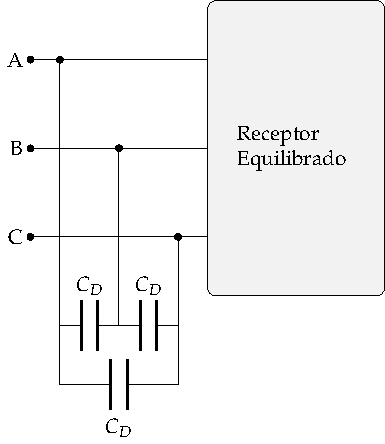
\includegraphics[width=.8\linewidth]{../figs/CircuitoTrifasica_CompensacionReactiva.pdf}
\end{center}
\end{column}
\end{columns}
\end{frame}

\begin{frame}{Mejora del factor de potencia}{Conexión en estrella}
\begin{columns}
\begin{column}{0.5\linewidth}
\begin{itemize}
\item En trifásica existen dos posibilidades:
\begin{itemize}
\item Conexión en triángulo (\(C_D\))
\item Conexión en estrella (\(C_Y\))
\begin{align*}
  Q &= P\tan\theta\\
  Q' &= P\tan\theta' = Q - Q_c\\
  Q_c &= 3 \, \omega C_Y \, U_F^2 = {3} \omega \,C_Y \left(\dfrac{U_L}{\sqrt{3}}\right)^2=\omega C_Y \, U_L^2
\end{align*}
\[
  \boxed{C_Y = \frac{P(\tan \theta - \tan \theta')}{\omega U_L^2}}
\]
\end{itemize}
\end{itemize}
\end{column}
\begin{column}{0.5\linewidth}
\begin{center}
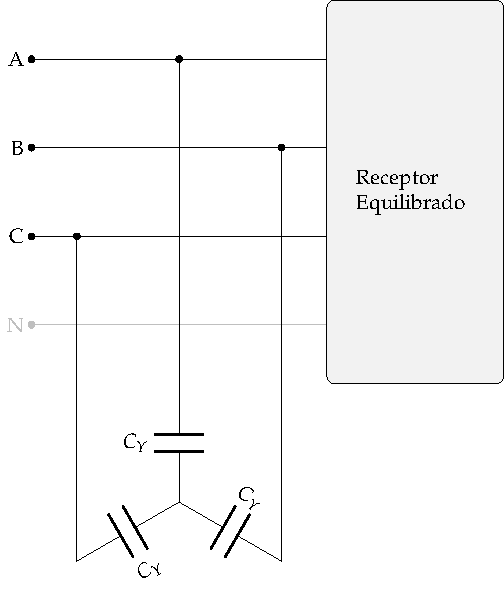
\includegraphics[width=.9\linewidth]{../figs/CircuitoTrifasicaY_CompensacionReactiva.pdf}
\end{center}
\end{column}
\end{columns}
\end{frame}

\begin{frame}{Mejora del factor de potencia}{Comparación Estrella-Triángulo}
\begin{columns}
\begin{column}{0.5\columnwidth}
\begin{center}
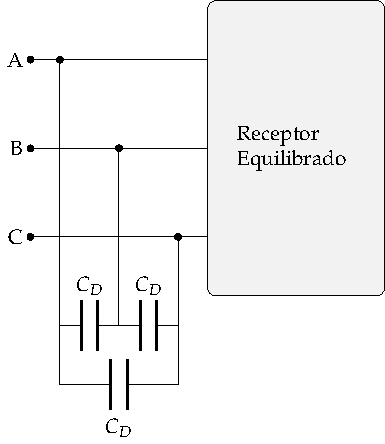
\includegraphics[height=0.55\textheight]{../figs/CircuitoTrifasica_CompensacionReactiva.pdf}
\end{center}
\[
  \boxed{C_D = \frac{P(\tan \theta - \tan \theta')}{3 \omega U^2}}
\]
\end{column}

\begin{column}{0.5\columnwidth}
\begin{center}
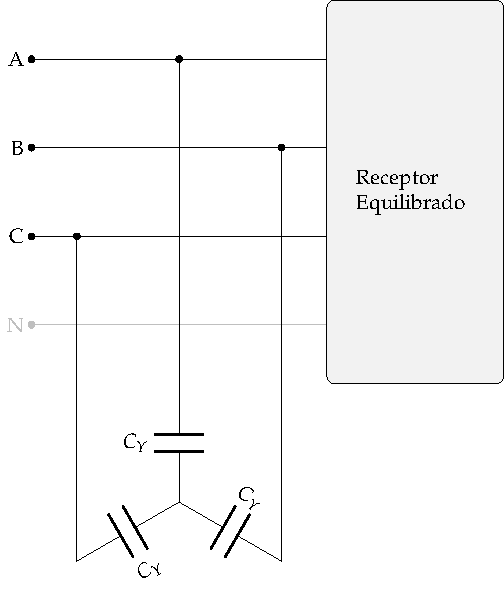
\includegraphics[height=0.55\textheight]{../figs/CircuitoTrifasicaY_CompensacionReactiva.pdf}
\end{center}
\[
  \boxed{C_Y = \frac{P(\tan \theta - \tan \theta')}{\omega U^2}}
\]

\medskip
\end{column}
\end{columns}

Dado que \(C_Y = 3 \cdot C_D\) la \alert{configuración recomendada} es \alert{triángulo}
\end{frame}

\begin{frame}{Mejora del factor de potencia}{Ejemplo}
    \textbf{Una red trifásica de 380 V, 50 Hz y secuencia SFD alimenta a dos cargas equilibradas: $(i)$ 30 kW y factor de potencia $0.7$ inductivo; $(ii)$ 24 kW y factor de potencia $0.6$ inductivo. Determinar la capacidad de cada uno de los condensadores a conectar a la red para que el factor de potencia global mejore hasta $0.95$.}
\end{frame}

\end{document}